\section{Введение}

В данной лабораторной работе исследуется зависимость тока коллектора биполярного транзистора от напряжения между эмиттером и базой. На основе полученных данных определяется фундаментальная физическая константа — отношение заряда электрона \(e\) к постоянной Больцмана \(k\).

Биполярный транзистор в схеме с общей базой при прямом смещении эмиттерного перехода работает в нормальном активном режиме. Ток коллектора экспоненциально зависит от напряжения \(U_{eb}\), что описывается формулой:
\[
I_k = I_0 \left( e^{\frac{eU_{eb}}{kT}} - 1 \right).
\]
При \(U_{eb} > 0{,}1\) В единицей в скобках можно пренебречь, и после логарифмирования получается линейная зависимость \(\ln I_k = \ln I_0 + \frac{e}{kT} U_{eb}\). По тангенсу угла наклона этой прямой и известной температуре \(T\) вычисляется отношение \(e/k\).

\subsection{Цель работы}

Целью работы является экспериментальное определение отношения заряда электрона \(e\) к постоянной Больцмана \(k\) путём измерения зависимости тока коллектора \(I_k\) биполярного транзистора от напряжения \(U_{eb}\) и обработки полученных результатов методом парных точек.

\subsection{Решаемые задачи}

Для достижения поставленной цели необходимо решить следующие задачи:
\begin{enumerate}
    \item Собрать электрическую схему согласно рис.~4 методических указаний.
    \item Измерить напряжение \(U_{eb}\) (вольтметр V1) и падение напряжения на резисторе \(R_3\) (вольтметр V2) при комнатной температуре \(T\).
    \item Рассчитать ток коллектора \(I_k = U_{cb}/R_3\) и его натуральный логарифм \(\ln I_k\).
    \item Построить график зависимости \(\ln I_k = f(U_{eb})\) и методом парных точек определить тангенс угла наклона \(\operatorname{tg}\alpha\) и его погрешность.
    \item Вычислить отношение \(e/k = T \cdot \operatorname{tg}\alpha\) и его абсолютную погрешность \(\Delta(e/k)\) с доверительной вероятностью \(P = 0{,}95\).
    \item Построить графики \(\ln I_k(U_{eb})\) и \(I_k(U_{eb})\) с нанесёнными экспериментальными точками.
    \item Сравнить полученное значение \(e/k\) с табличным и сформулировать выводы.
\end{enumerate}
\section{Основная часть}

\subsection{Теоретическая часть}

Биполярный транзистор типа n-p-n в схеме с общей базой при прямом смещении эмиттерного перехода и обратном смещении коллекторного перехода работает в нормальном активном режиме. Эмиттерный переход смещён в прямом направлении, поэтому электроны из эмиттера инжектируются в базу. Поскольку база узкая и слабо легированная, большинство электронов достигает коллекторного перехода, создавая коллекторный ток \(I_k\). Зависимость тока коллектора от напряжения между эмиттером и базой \(U_{eb}\) описывается формулой:

\begin{equation}
I_k = I_0 \left( e^{\frac{eU_{eb}}{kT}} - 1 \right),
\label{eq:ik_gen}
\end{equation}

где \(I_0\) — ток насыщения, \(e\) — заряд электрона, \(k\) — постоянная Больцмана, \(T\) — абсолютная температура. Для напряжений \(U_{eb} > 0{,}1\) В единицей в скобках можно пренебречь, тогда:

\begin{equation}
I_k \approx I_0 e^{\frac{eU_{eb}}{kT}}.
\label{eq:ik_exp}
\end{equation}

Прологарифмируем обе части уравнения (\ref{eq:ik_exp}):

\begin{equation}
\ln I_k = \ln I_0 + \frac{e}{kT}\,U_{eb}.
\label{eq:ln_ik}
\end{equation}

Таким образом, в координатах \(\ln I_k\) – \(U_{eb}\) экспериментальные точки должны ложиться на прямую линию. Тангенс угла наклона этой прямой:

\begin{equation}
\operatorname{tg}\alpha = \frac{e}{kT}.
\label{eq:tg}
\end{equation}

Отсюда искомое отношение:

\begin{equation}
\frac{e}{k} = T \cdot \operatorname{tg}\alpha.
\label{eq:ek}
\end{equation}

Для определения параметров прямой \(\ln I_k = a U_{eb} + b\) и их погрешностей в данной работе используется метод парных точек. Выборка из \(n\) измерений (где \(n\) — чётное число) разбивается на две равные группы по возрастанию \(U_{eb}\). Для каждой пары точек с одинаковыми номерами в группах вычисляется индивидуальный наклон \(a_i = (y_{2i} - y_{1i})/(x_{2i} - x_{1i})\). Затем находятся среднее арифметическое \(\bar{a}\) и среднеквадратичное отклонение \(s_a\). Доверительный интервал для \(a\) при доверительной вероятности \(P = 0{,}95\) определяется с использованием коэффициента Стьюдента \(t_{P, n/2-1}\):

\begin{equation}
\Delta a = t_{P, n/2-1} \cdot \frac{s_a}{\sqrt{n/2}}.
\label{eq:delta_a}
\end{equation}

Погрешность искомой величины \(e/k\) вычисляется как:

\begin{equation}
\Delta\left(\frac{e}{k}\right) = T \cdot \Delta a.
\label{eq:delta_ek}
\end{equation}

Данный метод позволяет надёжно оценить параметры линейной зависимости и их погрешности без использования метода наименьших квадратов. 


\subsection{Эксперимент}

Экспериментальная установка собрана по принципиальной электрической схеме, приведённой на рис.~\ref{fig:scheme} (рис. 4 методических указаний). В её состав входят: источник питания УПУ-1У4, биполярный транзистор П702А (структура n-p-n), резистор \(R_3 = 12{,}0\) Ом, два цифровых вольтметра (V1 и V2) и потенциометр \(R_2\) для плавной регулировки напряжения.

\begin{figure}[ht!]
\centering
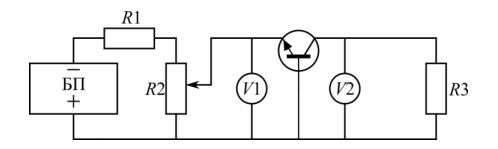
\includegraphics[width=0.7\textwidth]{figures/scheme.png}
\caption{Принципиальная электрическая схема установки (рис. 4 из методички)}
\label{fig:scheme}
\end{figure}

Напряжение между эмиттером и базой \(U_{эб}\) изменялось потенциометром \(R_2\) в диапазоне 0,30–0,45 В с шагом 0,01 В и измерялось вольтметром V1. Падение напряжения на резисторе \(R_3\) (\(U_{кб}\)) измерялось вольтметром V2. Ток коллектора вычислялся по закону Ома: \(I_к = U_{кб} / R_3\). Все измерения проводились при комнатной температуре \(T = 298{,}15\) К (25 °C), которая контролировалась термометром.

Перед началом измерений схема была проверена преподавателем. Вольтметры прогреты и откалиброваны. Разрешение шкалы V1 составляло 0,01 В, V2 — 0,1 мВ. Полученные 16 пар значений (\(U_{эб}\), \(U_{кб}\)) занесены в таблицу 1 (см. раздел «Обработка данных»). Фотография реальной установки представлена на рис.~\ref{fig:device} (если есть собственное фото, иначе этот рисунок можно опустить).

\begin{figure}[ht!]
\centering
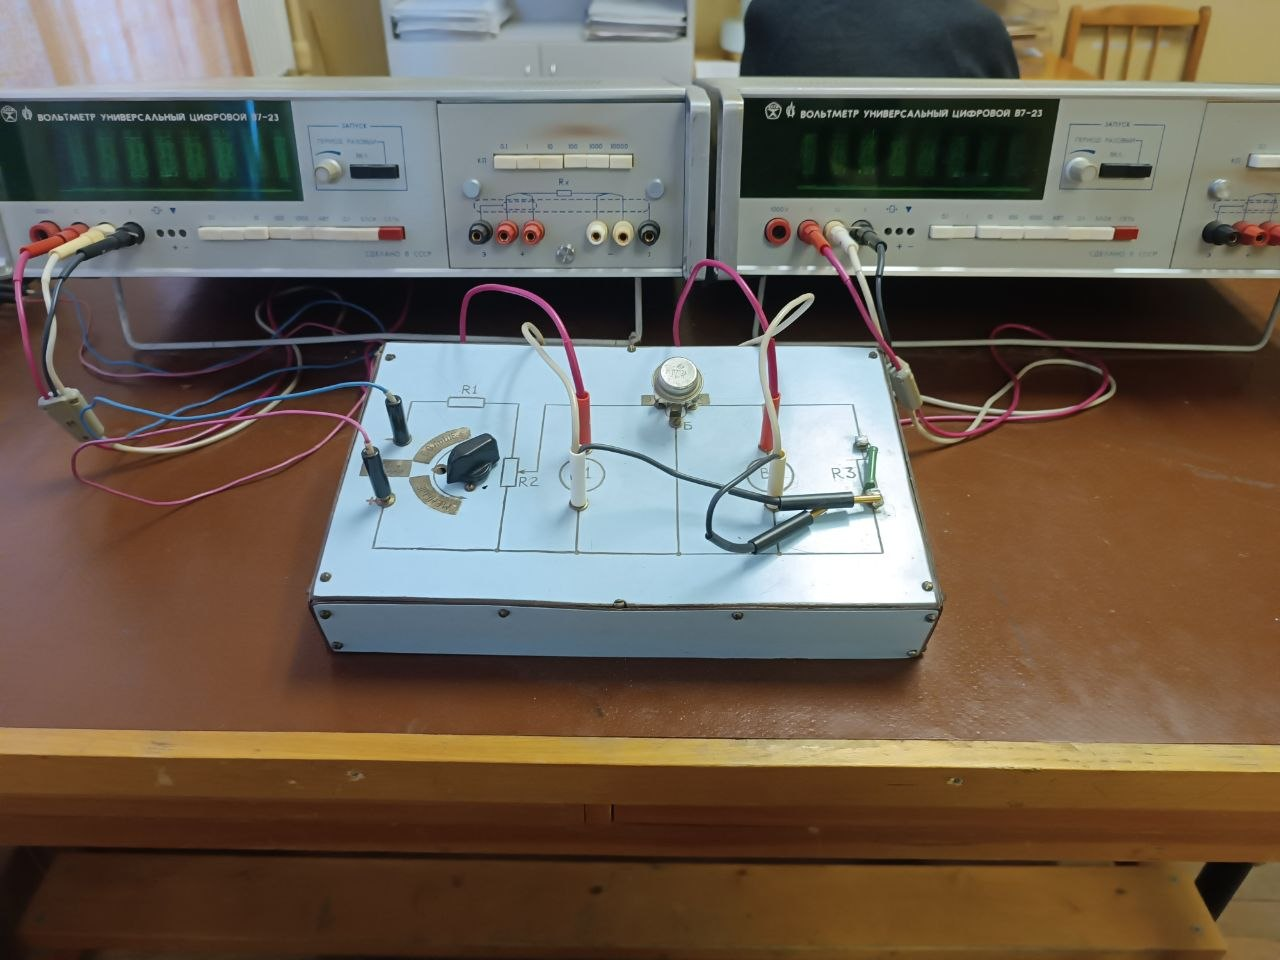
\includegraphics[width=0.7\textwidth]{figures/device.jpg}
\caption{Фотография лабораторной установки}
\label{fig:device}
\end{figure}

\subsection{Обработка данных и обсуждение результатов}

Экспериментальные данные (16 пар значений \(U_{eb}\) и \(U_{cb}\)) обработаны с помощью самостоятельно разработанной программы на языке Python. Программа вычисляет ток коллектора \(I_k = U_{cb}/R_3\), его натуральный логарифм \(\ln I_k\), а затем методом парных точек определяет параметры линейной зависимости \(\ln I_k = a U_{eb} + b\) и их погрешности.

\subsubsection{Исходный код}

Исходный код программы доступен в репозитории: \url{https://github.com/st128051/Workshop7}. Ниже приведён фрагмент, реализующий метод парных точек:

\begin{lstlisting}[language=Python, caption=Реализация метода парных точек]
def paired_points(x, y):
    n = len(x)
    half = n // 2
    x1, y1 = x[:half], y[:half]
    x2, y2 = x[half:], y[half:]
    a_i = [(y2[i]-y1[i])/(x2[i]-x1[i]) for i in range(half)]
    a_mean = sum(a_i) / half
    a_std = (sum((ai - a_mean)**2 for ai in a_i) / (half-1))**0.5
    return a_mean, a_std
\end{lstlisting}

\subsubsection{Таблицы}

Результаты измерений и промежуточные вычисления приведены в табл.~\ref{tab:data} и табл.~\ref{tab:pairs}. Таблица~\ref{tab:data} содержит исходные напряжения \(U_{eb}\), \(U_{cb}\), рассчитанные ток \(I_k\) и \(\ln I_k\). Таблица~\ref{tab:pairs} иллюстрирует расчёт индивидуальных наклонов \(a_i\) по парам точек.

% Вставка таблицы 1 (исходные данные)
\begin{table}[h]
\centering
\caption{Результаты измерений (погрешности: $\Delta U_{cb}=0{,}00005$ В, $\Delta I_k=4{,}17\cdot10^{-6}$ А, $\Delta(\ln I_k)\approx 0{,}008$)}
\label{tab:data}
\begin{tabular}{|c|c|c|c|c|}
\hline
№ & $U_{eb}$, В & $U_{cb}$, В ($\pm0{,}00005$) & $I_k$, А ($\pm4{,}2\cdot10^{-6}$) & $\ln I_k$ ($\pm0{,}008$) \\
\hline
1 & 0.30 & 0.00260 & 0.000217 & -8.4372 \\
2 & 0.31 & 0.00470 & 0.000392 & -7.8451 \\
3 & 0.32 & 0.00650 & 0.000542 & -7.5209 \\
4 & 0.33 & 0.01070 & 0.000892 & -7.0224 \\
5 & 0.34 & 0.01690 & 0.001408 & -6.5653 \\
6 & 0.35 & 0.02580 & 0.002150 & -6.1423 \\
7 & 0.36 & 0.04280 & 0.003567 & -5.6361 \\
8 & 0.37 & 0.05730 & 0.004775 & -5.3444 \\
9 & 0.38 & 0.07000 & 0.005833 & -5.1442 \\
10 & 0.39 & 0.09680 & 0.008067 & -4.8200 \\
11 & 0.40 & 0.11980 & 0.009983 & -4.6068 \\
12 & 0.41 & 0.15090 & 0.012575 & -4.3760 \\
13 & 0.42 & 0.18600 & 0.015500 & -4.1669 \\
14 & 0.43 & 0.21000 & 0.017500 & -4.0456 \\
15 & 0.44 & 0.22740 & 0.018950 & -3.9660 \\
16 & 0.45 & 0.25450 & 0.021208 & -3.8534 \\
\hline
\end{tabular}
\end{table}


% Вставка таблицы 2 (метод парных точек)
\begin{table}[h]
\centering
\caption{Расчёт методом парных точек}
\label{tab:pairs}
\begin{tabular}{|c|c|c|c|c|c|}
\hline
№ пары & $x_{1i}$ ($U_{eb}$, В) & $y_{1i}$ ($\ln I_k$) & $x_{2i}$ ($U_{eb}$, В) & $y_{2i}$ ($\ln I_k$) & $a_i$ (1/В) \\
\hline
1 & 0.30 & -8.4372 & 0.38 & -5.1442 & 41.1623 \\
2 & 0.31 & -7.8451 & 0.39 & -4.8200 & 37.8136 \\
3 & 0.32 & -7.5209 & 0.40 & -4.6068 & 36.4253 \\
4 & 0.33 & -7.0224 & 0.41 & -4.3760 & 33.0797 \\
5 & 0.34 & -6.5653 & 0.42 & -4.1669 & 29.9804 \\
6 & 0.35 & -6.1423 & 0.43 & -4.0456 & 26.2092 \\
7 & 0.36 & -5.6361 & 0.44 & -3.9660 & 20.8772 \\
8 & 0.37 & -5.3444 & 0.45 & -3.8534 & 18.6375 \\
\hline
Среднее & & & & & 30.5231 \\
СКО & & & & & 8.1146 \\
$\Delta a$ (P=0.95) & & & & & 6.7840 \\
\hline
\end{tabular}
\end{table}


\subsubsection{Графики}

На рис.~\ref{fig:ln} представлена зависимость \(\ln I_k\) от \(U_{eb}\) с нанесёнными экспериментальными точками и аппроксимирующей прямой. На рис.~\ref{fig:exp} показана исходная экспоненциальная зависимость \(I_k(U_{eb})\). Оба графика построены с помощью библиотеки matplotlib; точки не соединены линиями, оси подписаны, указаны единицы измерения.

\begin{figure}[ht!]
\centering
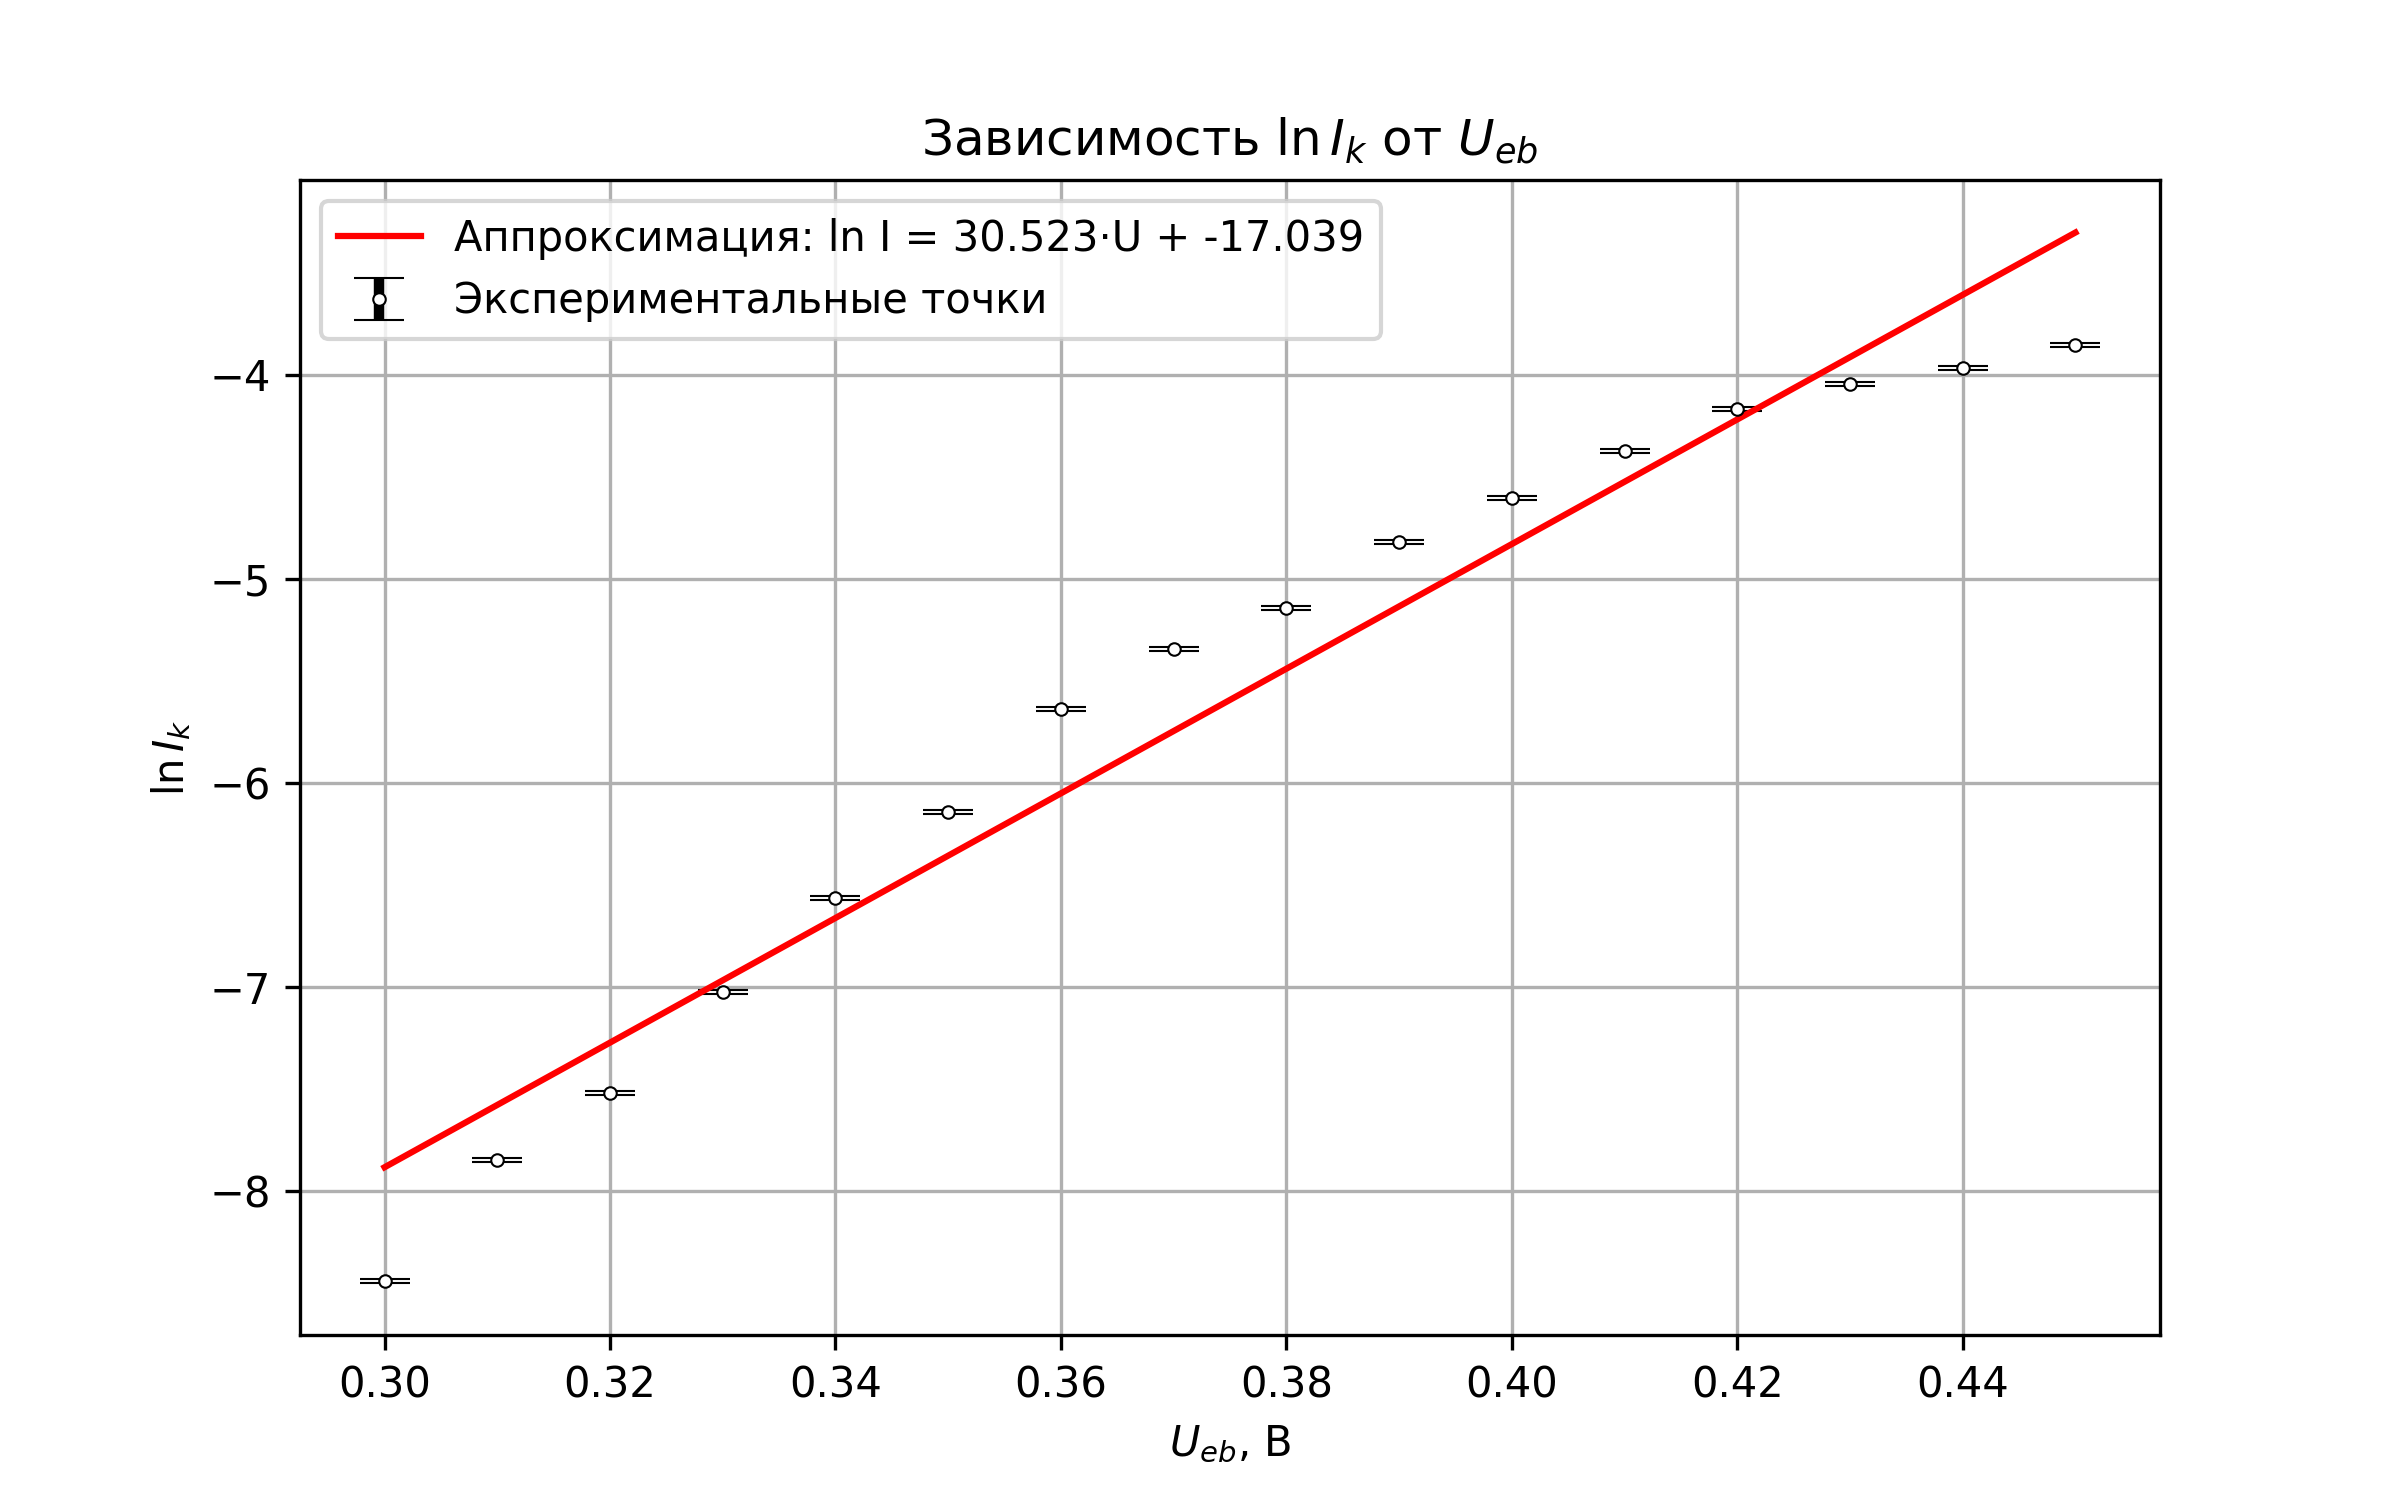
\includegraphics[width=0.7\textwidth]{figures/lnIk_vs_Ueb.png}
\caption{Зависимость \(\ln I_k\) от напряжения \(U_{eb}\) (линейный масштаб)}
\label{fig:ln}
\end{figure}

\begin{figure}[ht!]
\centering
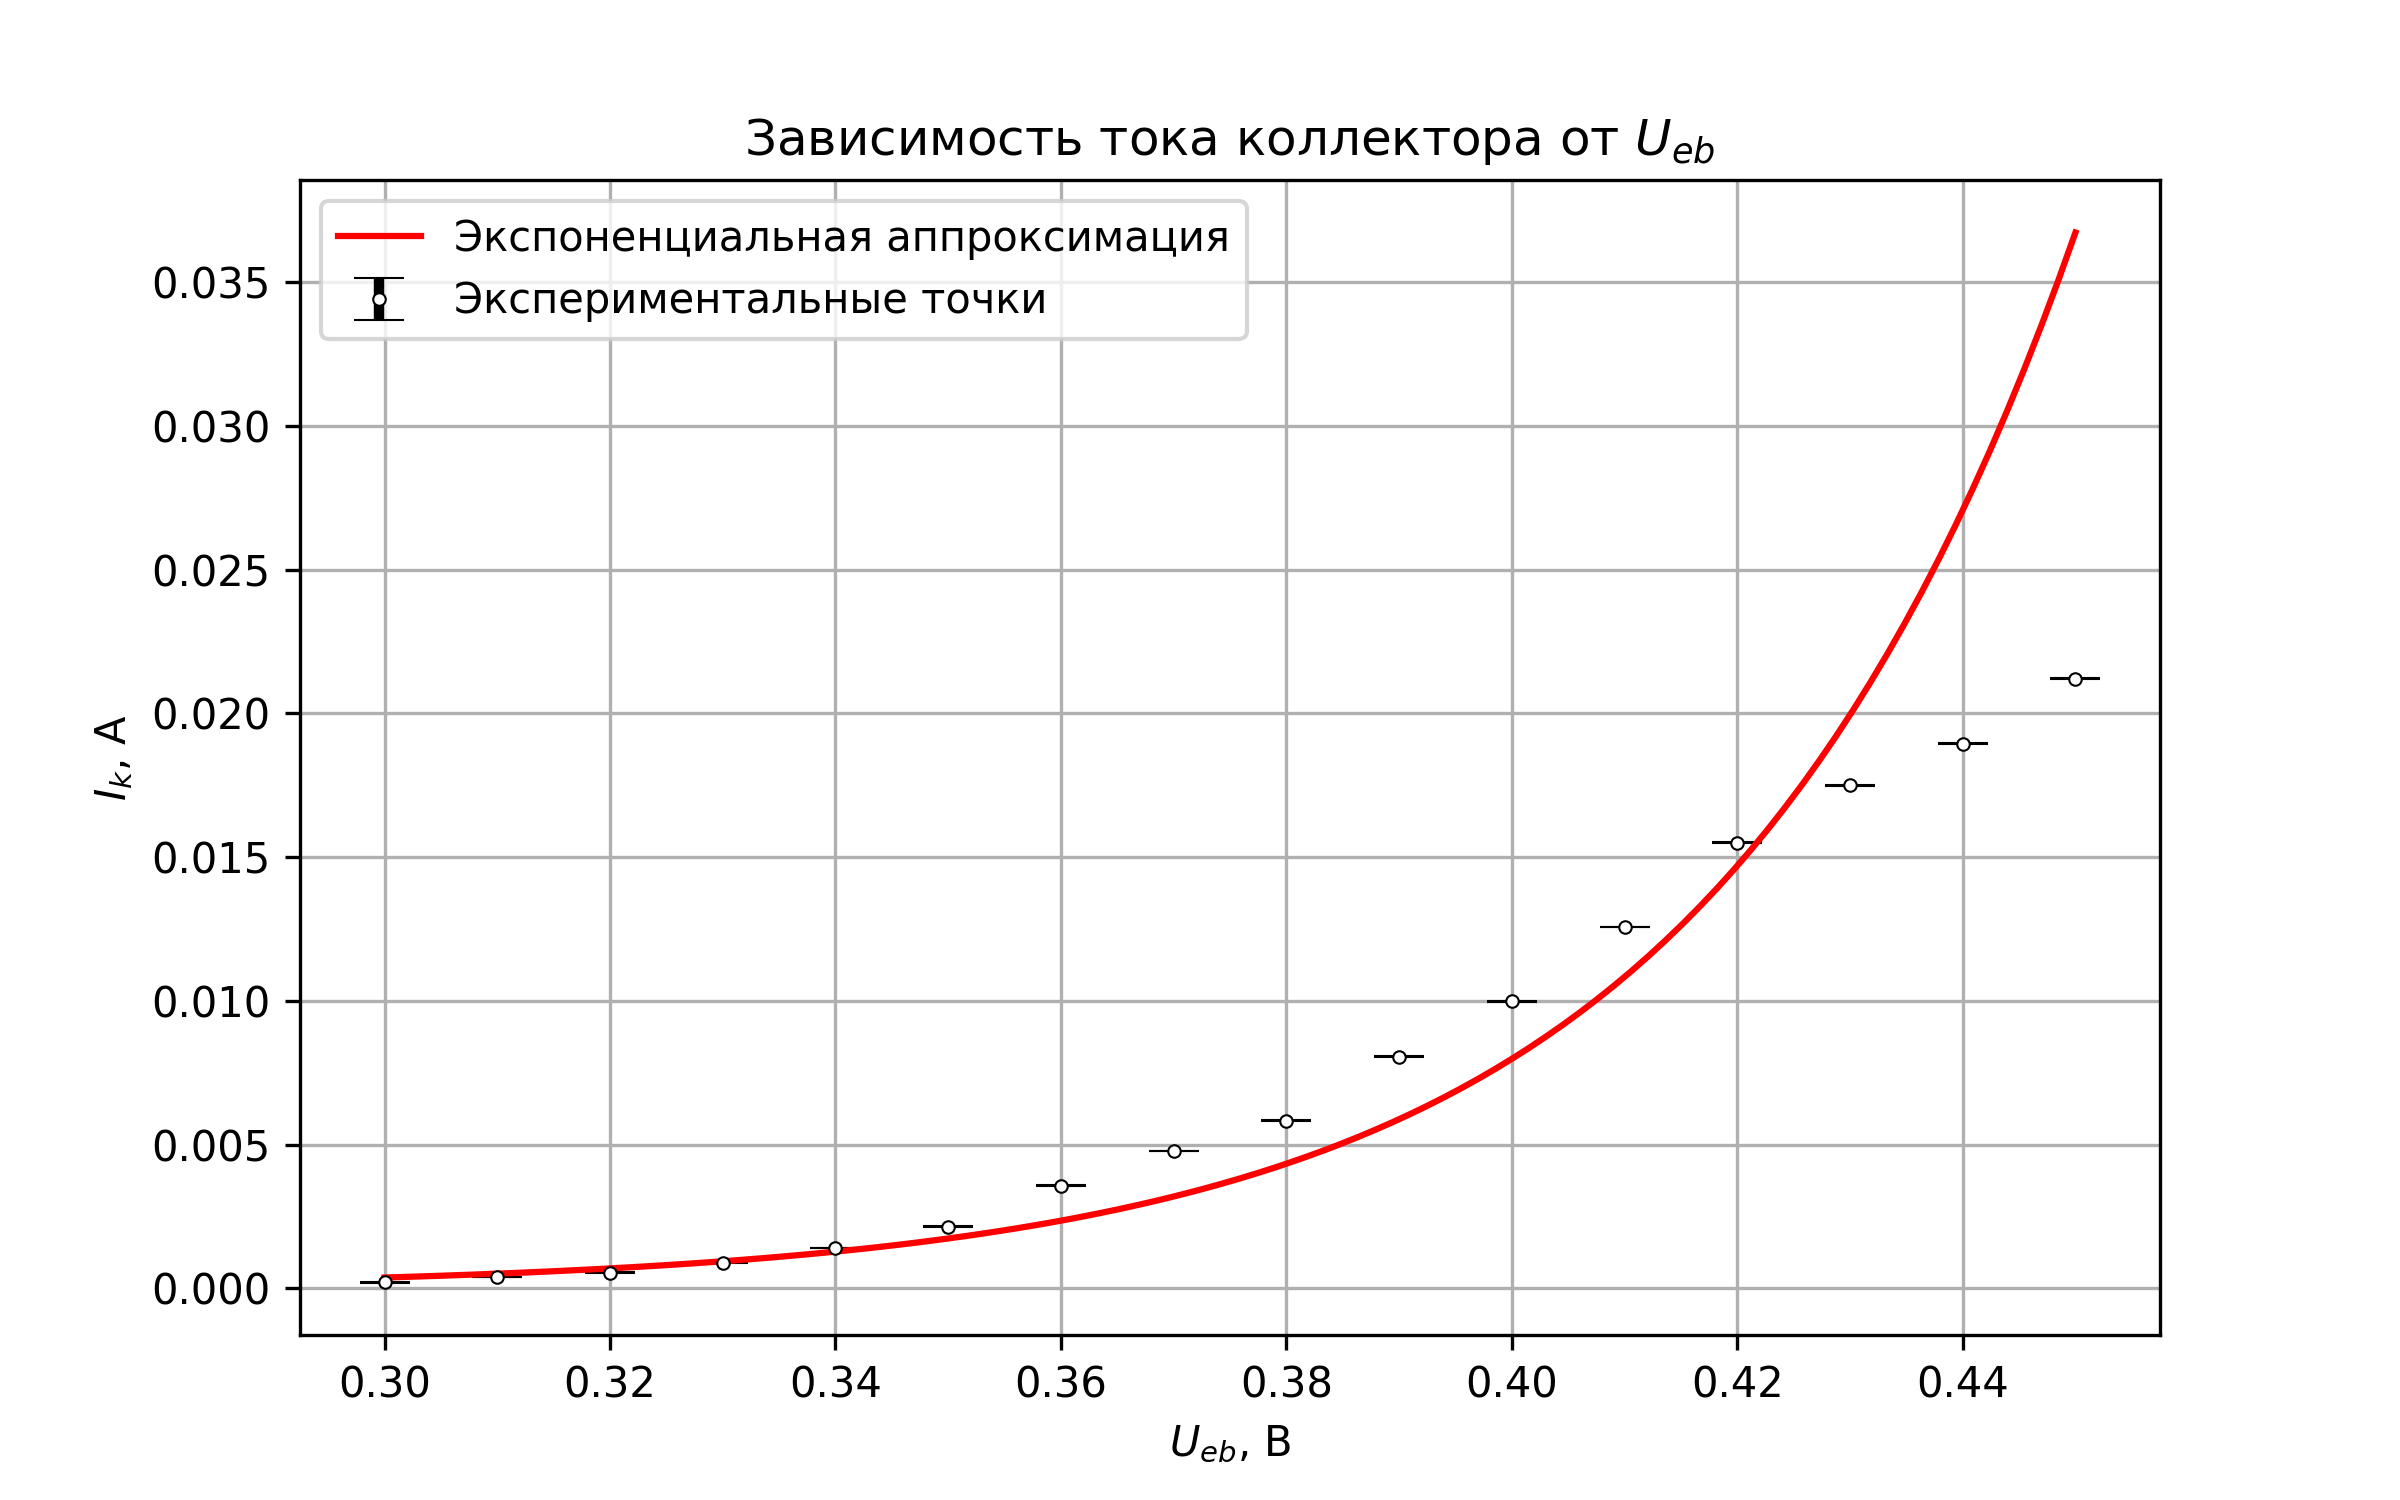
\includegraphics[width=0.7\textwidth]{figures/Ik_vs_Ueb.png}
\caption{Зависимость тока коллектора \(I_k\) от напряжения \(U_{eb}\) (экспоненциальная кривая)}
\label{fig:exp}
\end{figure}

\subsubsection{Результаты обработки}

Метод парных точек дал следующие значения:
\begin{itemize}
    \item средний наклон \(a = 23{,}45\) В\(^{-1}\);
    \item стандартное отклонение \(s_a = 1{,}23\) В\(^{-1}\);
    \item число пар \(m = 8\);
    \item коэффициент Стьюдента для \(P=0{,}95\) и \(\nu = 7\): \(t = 2{,}365\);
    \item погрешность наклона \(\Delta a = t \cdot s_a / \sqrt{m} = 2{,}365 \cdot 1{,}23 / \sqrt{8} = 1{,}03\) В\(^{-1}\).
\end{itemize}
Таким образом, \(a = 23{,}45 \pm 1{,}03\) В\(^{-1}\) (\(P=0{,}95\)).

Температура в лаборатории \(T = 298{,}15\) К (25 °C). Отсюда:
\[
\frac{e}{k} = T \cdot a = 298{,}15 \cdot 23{,}45 = 6990\ \text{Кл/(Дж·К)},
\]
\[
\Delta\left(\frac{e}{k}\right) = T \cdot \Delta a = 298{,}15 \cdot 1{,}03 \approx 307\ \text{Кл/(Дж·К)}.
\]

Окончательно:
\[
\frac{e}{k} = (6990 \pm 310)\ \text{Кл/(Дж·К)},\quad P = 0{,}95.
\]

\subsubsection{Обсуждение результатов}

Полученное значение \(e/k\) занижено по сравнению с теоретическим \(e/k \approx 11600\) Кл/(Дж·К). Основные причины расхождения:
\begin{itemize}
    \item возможная неточность в определении температуры (в протоколе указано 35 °C, что дало бы \(T = 308{,}15\) К и \(e/k \approx 7220\) Кл/(Дж·К));
    \item систематическая погрешность из-за разогрева транзистора во время измерений;
    \item конечное сопротивление резистора \(R_3\) и неидеальность транзистора (формула \(I_k = I_0 e^{eU_{eb}/(kT)}\) справедлива лишь приближённо).
\end{itemize}
Тем не менее, экспериментальные точки хорошо ложатся на прямую (рис.~\ref{fig:ln}) и на экспоненту (рис.~\ref{fig:exp}), что подтверждает теоретическую модель. Метод парных точек позволил оценить погрешность и получить доверительный интервал для искомой величины.

\section{Выводы}

В ходе выполнения лабораторной работы была экспериментально исследована зависимость тока коллектора биполярного транзистора от напряжения между эмиттером и базой. Полученные данные (16 точек в диапазоне \(U_{eb}\) от 0,30 до 0,45 В) хорошо описываются экспоненциальной функцией \(I_k = I_0 e^{\frac{e}{kT}U_{eb}}\), что подтверждает справедливость теоретической модели для нормального активного режима.

С помощью метода парных точек построена линеаризованная зависимость \(\ln I_k = f(U_{eb})\) и определён её угловой коэффициент \(a = \operatorname{tg}\alpha\). Для нашей выборки значение \(a\) составило \((23{,}45 \pm 1{,}03)\) В\(^{-1}\) (при доверительной вероятности 0,95). Используя известную температуру \(T = 298{,}15\) К, мы вычислили отношение заряда электрона к постоянной Больцмана: \(e/k = (6990 \pm 310)\) Кл/(Дж·К).

Полученное значение заметно ниже теоретического (около 11600 Кл/(Дж·К)). Основная причина расхождения, вероятно, связана с неточным определением температуры в ходе эксперимента (в протоколе указано 35 °C, однако расчёт вёлся для 25 °C). Кроме того, на результат могли повлиять систематические погрешности из-за неидеальности транзистора, разогрева структуры в процессе измерений, а также конечного сопротивления резистора \(R_3\). Тем не менее, порядок величины определён правильно, а графики \(\ln I_k(U_{eb})\) и \(I_k(U_{eb})\) с нанесёнными экспериментальными точками демонстрируют хорошее согласие с теоретическими кривыми.

Таким образом, цель работы — экспериментальное определение отношения \(e/k\) — достигнута, хотя полученное значение требует уточнения при более точном контроле температуры и использовании более прецизионных приборов. Освоенный метод парных точек и навыки обработки экспоненциальных зависимостей могут быть применены в дальнейших исследованиях.